%%% Architecture section

\section{Monitoring Architecture}
There are many proposed architectures for use in runtime monitoring. Fundamental questions such as where the monitor executes (e.g., external hardware or on-system), what the monitor watches (e.g., memory values, executed instructions, etc.) and how the monitor obtains input (e.g., system instrumentation, external sensors) are dependent on both the properties of the system being monitored and the desired effects of monitoring (i.e., observation or enforcement/control).  

Existing runtime monitoring techniques tend to clash with the constraints imposed by safety-critical embedded systems. 
Most current proposed monitors rely on automatic generation of instrumentation code or generation of the monitor itself (e.g., \cite{Havelund2002, Pike2011}).
This is unusable in black box or external supplier scenarios due to the lack of source code access and has a greater chance of affecting the non-faulty system behavior, especially timing in real-time systems.
Instead, we proposes a passive external monitor which only checks system properties that are observable by watching a broadcast network.
%These include not only direct constraints including cost sensitivity and real-time computation but also development constraints such as system certification and source code access for black-box components.
Although we focus on ground vehicles and CAN in this work, other similar systems can also be monitored with this approach due to the flexible interface and system model.
For example, Systems without broadcast buses may be monitored by exposing the desired system state to the monitor (either through instrumentation or intelligent monitor placement such as network gateways/routers).

\subsection{Arch Outline}
An outline of our monitor architecture is shown in Figure \ref{fig:architecture}. The monitor is connected to the target system on its broadcast bus. This bus is connected to the semi-formal interface which observes the bus traffic and generates atomic propositions for the monitor based on the observed bus state, building a system state snapshot for the monitor. 
The trace that is formally monitored is a series of these snapshots. The monitor algorithm takes the target specification $\varphi$ and the trace step generated by the semi-formal mapping $\sigma_i$ and outputs whether the current trace satisfies or violates the given specification. 
This output is sent to an action controller, which chooses the desired action based on the monitor results. Possible actions include logging violations and activating warnings for passive monitors or triggering a recovery action such as a safety shutdown for more active monitors.

%The target system is monitored by filtering the observable system state through a semi-formal mapping which produces the system trace $\sigma$. 
%This trace, along with the desired system specification $\varphi$ is provided to the formal monitoring algorithm \agmon\ which outputs whether the system trace satisfies or violates the given specification. This output can then be used to trigger a warning or perform some other recovery action as desired.

\begin{figure}
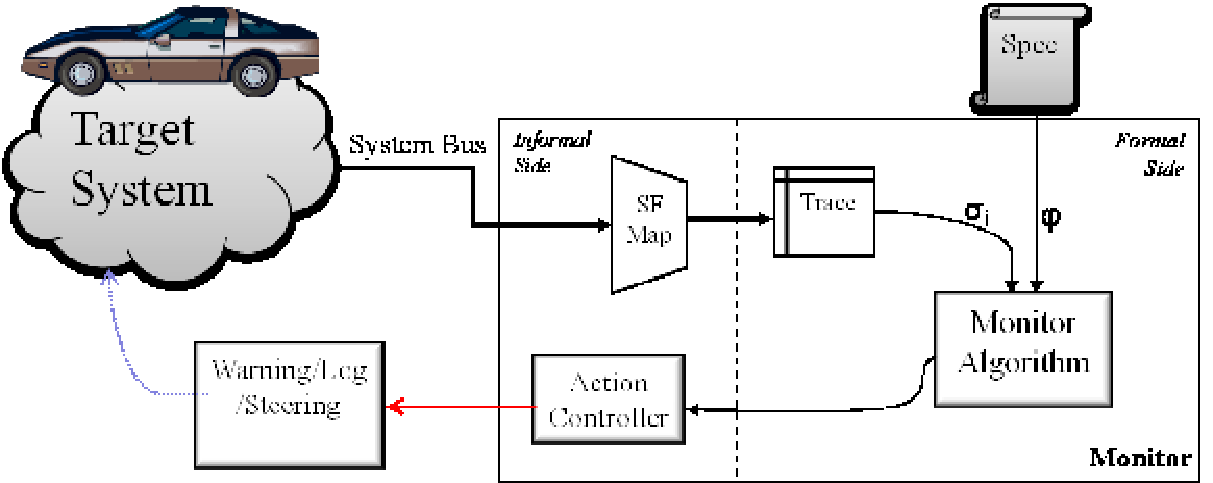
\includegraphics[width=4.5in]{img/mon_arch}
\caption{External monitor architecture outline \label{fig:architecture}}
\end{figure}

This architecture separates the system-independent formal aspects of the monitor from the system-dependent components including the semi-formal interface and system configurations. 
%By utilizing a semi-formal interface, we can separate the formal aspects of the monitor, which are completely independent from the target system, from the more practical pieces: the monitor interfaces and their configurations, which are system dependent. 
This allows us to utilize a core formal monitoring algorithm and framework with any system where an interface map can be used to create a state snapshot. 
Separating the system dependent and system-independent aspects of the monitor also lets the high level system requirements be somewhat abstracted away from the implementation. This means that changes to the target system may only require changes to the interface configuration and not the high level system specification. This is a similar situation to the two-level specifications used in the MaC framework \cite{Kim2004}.

\subsection{Semi-formal Monitoring}
Using formal methods has some clear benefits such as removing ambiguity, enabling early defect identification and allowing automated checking of properties. Even so, industrial adoption of formal methods, especially in software and system engineering has been slow (with hardware design being an exception) due to well known challenges such as a lack of tools and difficulty integrating with real systems \cite{Knight1998}. 
%
With regards to formal specifications, one possible cause is that completely describing a real system in most formal languages can be difficult or imposible. This is a part of Knight et al's formal specification evaluation criteria \emph{coverage}, which notes that a formal specification must permit description of all of an application or be designed to operate with any other notations that will be required \cite{Knight1997a}. 
This is a key concept for any practical and general runtime verification framework for real-world systems. Different systems will have varying specification needs, and if these needs are not easily met history shows that system designers are likely to just use an informal specification instead, which restricts the use of formal verification techniques.

To ensure specification flexibility, we have implemented a semi-formal specification which combines a formal specification with a semi-formal \emph{system mapping} which translates the actual system values into the monitor's more abstract execution trace. 
This semi-formal interface allows considerable leeway in designing the translation between the system and monitor's model. This leeway is both powerful and potentially dangerous. 
By allowing certain transformations in the interface, we are able to remove complexity from the monitor itself while ensuring that we can monitor a diverse set of needs.
This approach needs to be used carefully because it shifts part of the specification away from being formally defined, creating more opportunity for design mistakes and eroding some of the benefits that lead us to formal runtime verification in the first place.

%@PHIL need figure that summarizes this section
The two part specification feeds into two parts of the monitor, as shown in Figure \ref{fig:arch:arch_config}. 
The high-level formal specification contains the formal logic formulas that are directly checked by the formal monitoring algorithm.
The lower-level semi-formal mapping is used to define the system to monitor interface which generates the formal trace propositions that are checked by the monitoring algorithm. From an framework perspective, the semi-formal interface has minimal design constraints. 
As long as the interface provides a system trace of the properties present in the formal specification, we do not restrict how this trace is created.
%The interface can do any complex computations as long as it provides a system trace of the properties present in the formal specification. 

\begin{figure}
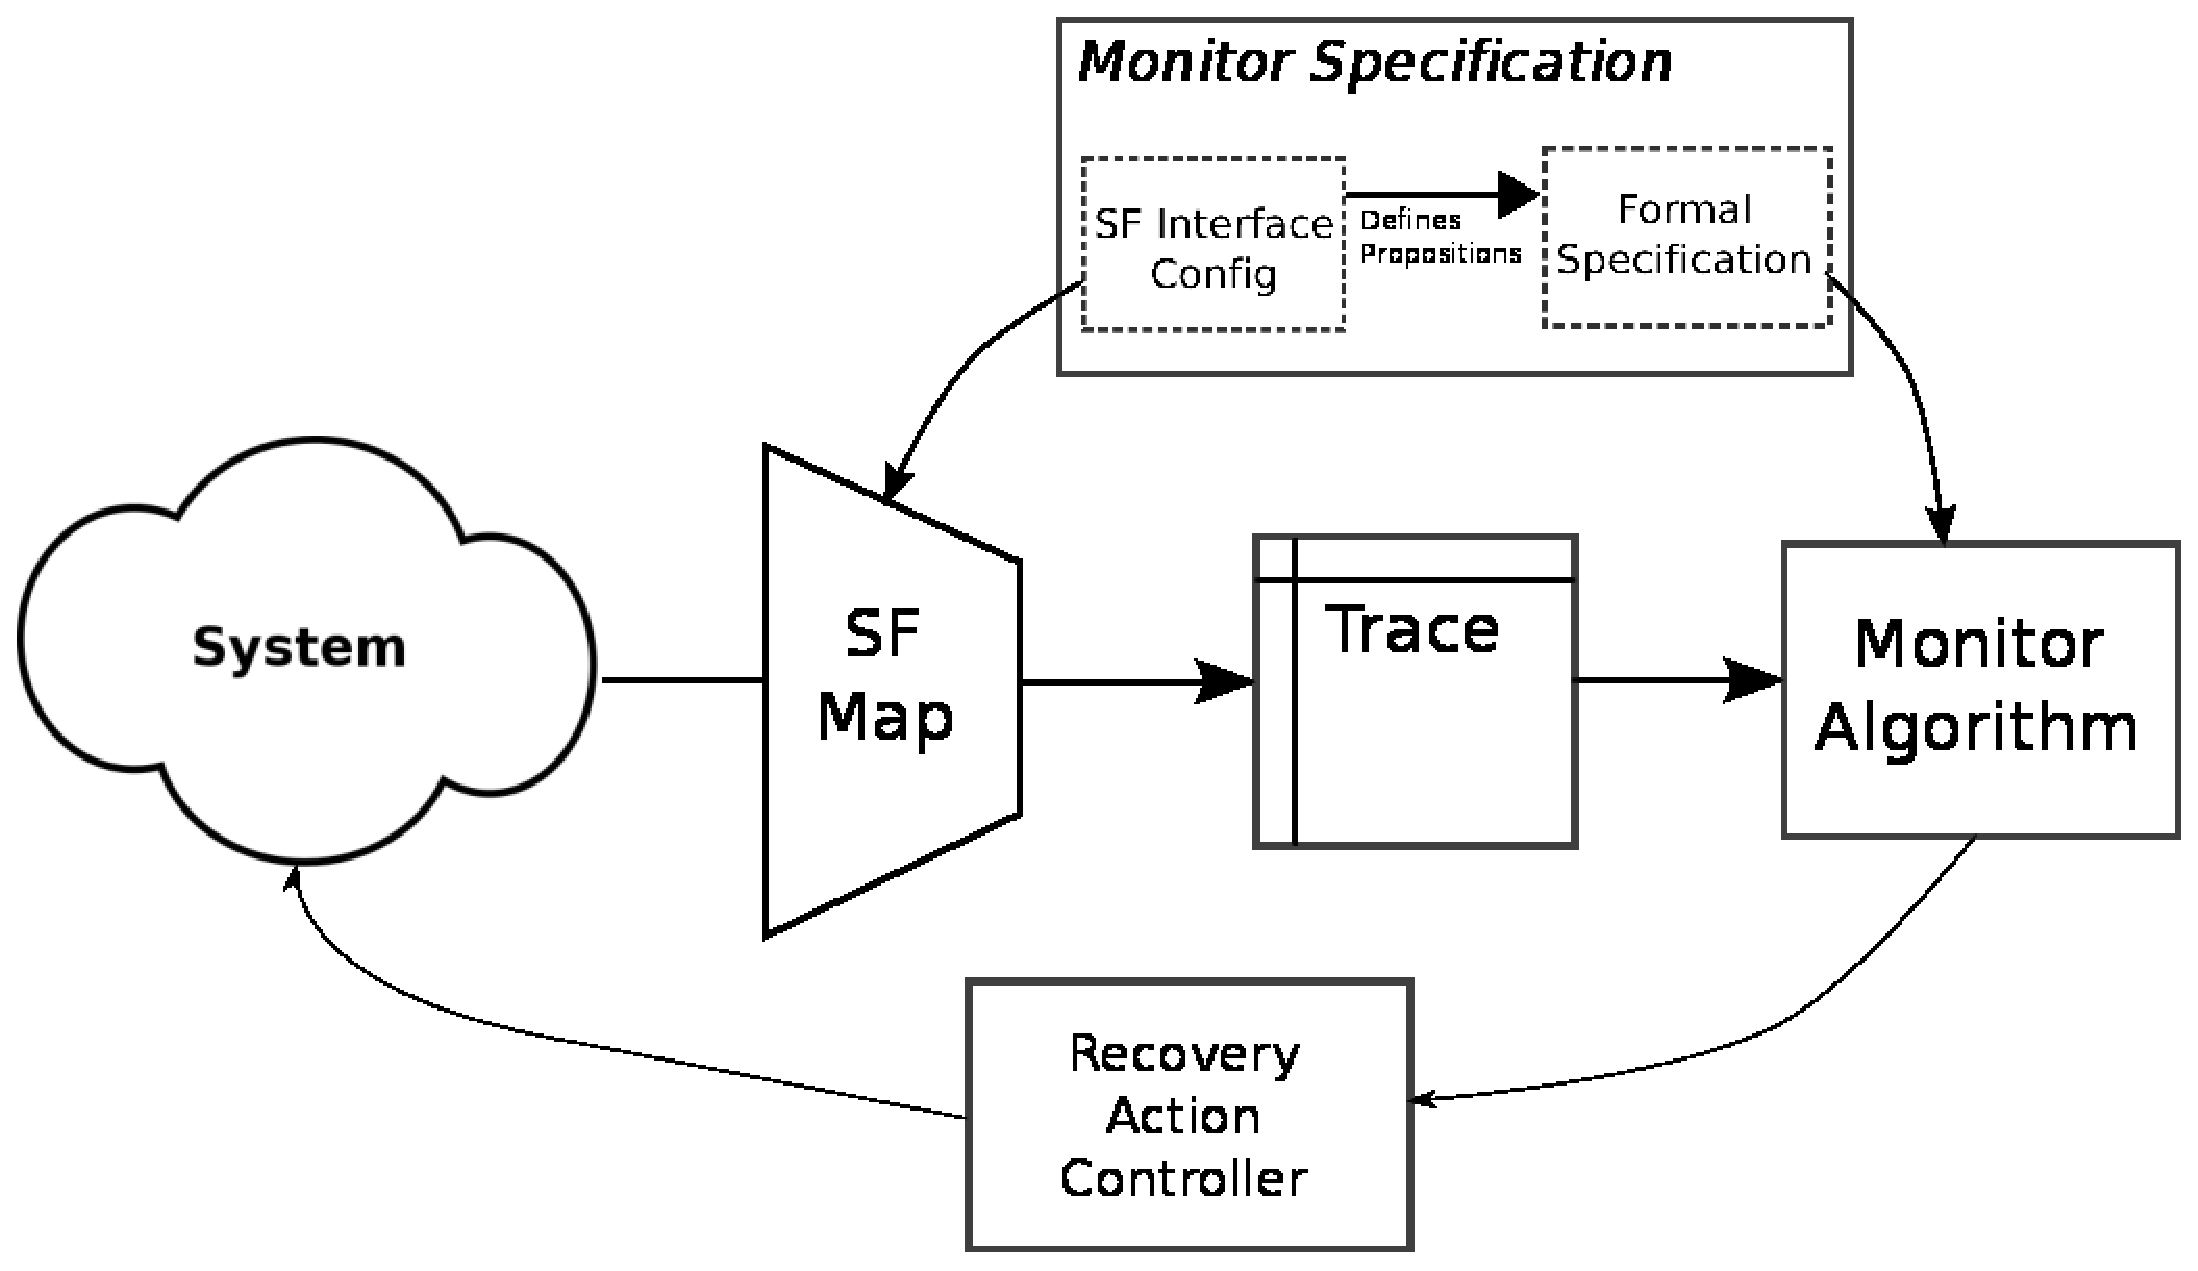
\includegraphics[width=4.5in]{img/arch_config}
\caption{Monitor architecture showing multi-part specification \label{fig:arch:arch_config}}
\end{figure}
Because the correctness of the monitor ultimately relies on the correctness of the interface transformations, limiting the interface to a simple, verifiable set of transformations is key to providing guarantees about the monitor's output.

The interface has two primary purposes: 

\begin{enumerate}
	\item To convert actual system values (e.g., network message data) into a propositional execution trace. 
	%\item To map these network messages onto specification propositions
	\item To provide additional semantic power to create useful propositions (e.g., state machines).
\end{enumerate}

The interface translates observable system state into a trace of propositions which can be checked against a specification by our monitoring algorithm. 
%
The interface provides the ability to extract the relevant data out of network messages in a flexible, network agnostic way. It can be used to extract the desired portion of a message, change units or typecast as necessary and then store the created proposition value correctly for use with the monitor. This ensures that the monitor is not restricted to networks or message types that it already knows how to transform. Any necessary data transformations can also be done in the interface.
%
Besides simple transformations (e.g., storing boolean values into propositions, arithmatic comparisons, etc.), we can also do more complex compututations and conversions in the interface such as building state machines whose state can be used to fill propositions.
%Besides relatively obvious transformations (status booleans into propositions, arithmatic comparisons) we can also do some slightly more complex computing in the interface such as building state machines and providing their value as a proposition.

%\subsection{Semi-Formal Interface Design}
The semi-formal interface is used provide the monitoring algorithm with the state trace.
There are no inherent limitations on the semi-formal interface besides that it must create a viable trace for the monitor.
%As long as it provides the monitoring algorithm a viable state, the monitor will work. 
There is, however, a practical limitation -- the more complex the interface becomes the less confidence we should have that it works correctly.
Given this, we'd like to restrict the interface as much as possible while still providing the necessary flexibility.
% so we 

From our experience with system requirements and monitoring, the important transformations that are common for these types of systems are simple arithmetic, boolean connectives, comparisons to recent values, and simple state machines. 
%
Because of this, we restrict our own semi-formal mapping syntax to a simplified subset of the C programming language. We allow all the basic algorithmic, bitwise, and comparison operators and statically allocated variables of primitive types (i.e., integers, floating point).
We do allow simple loops, for example over a static array holding a set of values, for calculating averages and other simple values.
We do not currently have a formal definition of the semi-formal syntax, instead we trust that users can decide how restricted they wish to and realistically can be.

%Knowing this we can define a restricted semi-formal syntax based on the semantics of the C programming language, shown in Figure \ref{fig:arch:sfm_syntax}.
%
%Our monitor implementation's semi-formal mapping configuration is integrated into the monitor's code directly by a specification compiler. 
%This is essentially an internal domain specific language (DSL) \cite{Barringer2012}. 
%Using a DSL to specify the semi-formal mappings allows us to restrict the specification of the interface to keep verification (of the interface) reasonable while still providing the ease of use and power of a programming language. 
%Other prototype monitors we designed have used more traditional interface DSLs where the specifications have been used to insert and generate the code used by the monitor for the interface. 
%More discussion about using domain specific languages for the semi-formal interface is included in Section \ref{sec:discussion:dsl}.

%%%% sfm_syntax\ldots
%\begin{figure}
%var ::= int | bool | \ldots \\
%SFM ::= var | var+var | var*var | \ldots \\
%\caption{Restricted Semi-Formal interface syntax \label{fig:arch:sfm_syntax}}
%\end{figure}

% describe the syntax\ldots
The motivation behind the restricted interface syntax is to provide enough power to define the system propositions necessary to monitor any reasonable desired property while incentivizing the monitor designers to work within the formal specification as much as possible.
%
%%%%@RV Hiding all this from now, probably need to rewrite the entire section to make sense in a shorter way
%Given a desired set of system properties, it is easy to imagine the pathological case where the monitor is configured to check the proposition \texttt{SystemOK} and the interface is built to compute this value directly. While this technically would work, it is obviously an abuse of the interface and a bad (non?) use of the monitor framework. Doing this essentially creates a completely informal monitor inside the interface, wasting the proven correctness of the formal monitoring algorithm.
%
%A more interesting case is when we have a system message which includes a value and a validity bit (signifying whether the message value is valid). 
%We can imagine that most rules utilizing this value will want to check both some property of the value and whether it is valid at the same time (e.g., \texttt{valuePositive} and \texttt{valueValid}). 
%This could be done on the formal side in the logic by using $\texttt{valuePositive} \wedge \texttt{valueValid}$ or by combining them in interface into one proposition $\texttt{valuePositiveValid}$ which is calculated from both incoming values. 
%
%In this case it is less clear which method is superior, but we can suggest a few heuristics to help decide. Perhaps the most straightforward way to choose is to attempt to mirror the design documentation and requirements in the monitor specification. 
%If the system requirements mention the validity either explicitly (as a message value) or implicitly (by mentioning a ``valid positive value'') then the monitor specification should also directly mention validity and use the validity message value directly. 
%If the requirements do not mention validity, then we can treat validity as an implementation detail and hide it away in the interface's proposition transformation. 
%This follows the idea that the high-level requirements are abstracted away from the implementation. So if the validity bit is an artifact of the implementation then it is intuitive to deal with it in the interface, but if the validity bit is a part of the higher level system design then it should also be a part of the monitor specification.
%
%Other factors can also affect the decision, such as monitoring complexity (moving transformations to the interface can reduce the amount of work the monitoring algorithm has to do) or the desire to maximize the amount of monitoring that is formally performed. 
%These decisions should be kept consistent across specification rules to avoid confusion or misunderstanding.
In an ideal situation, the formal specification would contain all the relevant safety specification parts, leaving only the actual translation of system values to the semi-formal interface. 
There is an inherent trade-off between the complexity of the logic/model and the complexity of the semi-formal mapping. 
We use a stronger mapping with a less complex formal language to provide specification flexibility at the risk of mapping-caused problems. 
This provides the power to monitor essentially any observable system property, losing some formalisms as the properties become more complex.
%More complex translations than simple threshold comparisons or copying booleans may require some semi-formal transformation if the desired properties cannot be expressed in propositional logic. 
%The bare minimum transformations needed to build the necessary propositions should be used, keeping as much of the verification in the formal side as possible. 
%Moving parts of the transformation to the interface side is useful when necessary, but as the interface configuration complexity increases it becomes more important to validate and verify the interface itself.

%%@TODO mapping problems -- sampling periods and discrete value jumps
%% 	not sure if they go here or elsewhere, leaving note for now


%% andre notes
% system level spec is overapproximation? but! avoids the complexity of software
% what do people want from a semiformal map
%% can we say anything mathematically -- if you don't use something safe you don't have any guarantees


%%%%%%%%%%%%%%%%%%%%%%%%%%%%%%
%%% going to be way too long to copy without reformatting, but let's see
%%%%%%%%%%%%%%%%%%%%%%%%%%%%%%%%%%%%%%%

